%%%%%%%% ICML 2021 EXAMPLE LATEX SUBMISSION FILE %%%%%%%%%%%%%%%%%

\documentclass{article}

\usepackage{microtype}
\usepackage{subfigure}
\usepackage{booktabs}
\usepackage[dvips]{graphicx}
\usepackage{multirow,multicol}
\usepackage[table]{xcolor}
\usepackage{listings}
\usepackage{float}
\usepackage[export]{adjustbox}
\usepackage{amssymb}
\usepackage{amsfonts}
\usepackage{amsthm}
\usepackage{amsmath}
\usepackage{enumitem}
\usepackage{lipsum}
\usepackage{pdfpages}
\usepackage{xcolor} 
\usepackage{hyperref}
\usepackage[accepted]{icml2021}


\definecolor{codegreen}{rgb}{0,0.6,0}
\definecolor{codegray}{rgb}{0.5,0.5,0.5}
\definecolor{codepurple}{rgb}{0.58,0,0.82}
\definecolor{backcolour}{rgb}{255,255,255}

\lstdefinestyle{mystyle}{
    backgroundcolor=\color{backcolour},   
    commentstyle=\color{codegreen},
    keywordstyle=\color{magenta},
    numberstyle=\tiny\color{codegray},
    stringstyle=\color{codepurple},
    basicstyle=\ttfamily\footnotesize,
    breakatwhitespace=false,         
    breaklines=true,                 
    captionpos=b,                    
    keepspaces=true,                 
    numbers=left,                    
    numbersep=5pt,                  
    showspaces=false,                
    showstringspaces=false,
    showtabs=false,                  
    tabsize=2
}

\lstset{style=mystyle}

\graphicspath{{./}} 

% Attempt to make hyperref and algorithmic work together better:
%\newcommand{\theHalgorithm}{\arabic{algorithm}}

\begin{document}

\twocolumn[
\icmltitle{Reimplementation of the Classical Neural Ordinary Differential Equation \\
            Using Modern Computational Tools}

\begin{icmlauthorlist}
\icmlauthor{Wasif Ul Islam}{pu}
\end{icmlauthorlist}

\icmlaffiliation{pu}{School of Electrical and Computer Engineering, Purdue University, West Lafayette, Indiana USA}

\icmlkeywords{Machine Learning, ICML}

\vskip 0.3in
]

\printAffiliationsAndNotice{} % otherwise use the standard text.


\section{Introduction}
\label{submission}

Residual Neural Networks (RNN) provided a significant improvement on performance regarding deep
layered neural networks. The performance gains were obtained from introducing residual elements applied
to the ReLu operations within the hidden layer. This introduced robustness against the vanishing/exploding gradient
problem that most classical neural networks face \cite{19Shorten}.

However, there are some application of RNNs that still did not provide the ideal flexibility, in terms
of training models for data involving time-series data. Since RNNs have discrete hidden layers and residual
components to the ReLu operations performed to the hidden layers, it can interfere with learning dependencies
which are sensitive to time \cite{23Walther}.

A different class of neural networks look to satisfy the drawbacks that the previously mentioned network contain:
Neural Ordinary Differential Equations (NeuralODE). The prime benefit that NeuralODEs provide is it is naturally suited for modelling continuos
time data. In addition, it can provide computational flexibility in terms of configurability in forward-pass and backpropagation. 

This paper's objective is to provide a brief literature review into works that have enabled the use of NeuralODEs and discuss the
advantages and disadvantages related to the use of NeuralODEs. As many pieces of work focus on performance of NeuralODEs on time-series datasets,
a short experiment involving the classification of the MNIST dataset using a proof-of-concept NeuralODE model 
is presented along with comparisons of performance with a typical proof-of-concept implementation of a residual neural network.

\section{Related Works}

\subsection{Article: Neural Ordinary Differential Equations}

The concept of NeuralODEs have been discussed before the prescribed implementation by the paper
\textit{Neural Ordinary Differential Equations}. However, the primitive approach to the implementation of
NeuralODEs had very large computational resource consumption, to the point where training the model
on a substantial scale was not feasable. Since the NeuralODE consist of one continous layer with specific time steps
for numerical integration (Derivation of Neural ODE vs. Classical NN is explained further below), performing backpropagation
on NeuralODEs would be taking the gradient across each of the time steps. Since solving ODEs require small timesteps for accurate
representation of the dynamics that is being learned, ordinary back-propagation become as resource dependant as a ResNet with hundreds
of layers.

The major contribution for the respective paper is the adjoint sensitvity method, which allows for the back-propagation of
NeuralODE block at near constant space-complexity \cite{15He}. A comparison between a Recurrent Neural Network with 25
hidden-layers and the proposed NeuralODE architecture was presented with time-series data. 

\begin{figure}[H]
   \centering
   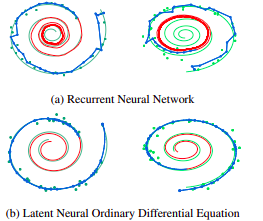
\includegraphics[width=0.75\linewidth]
   {./TimeSeries.png}
   \caption{Comparison Between Recurrent Neural Network and NeuralODE on Time-Series Data \cite{15He}}
   \label{fig:my_label}
\end{figure}

\subsection{Article: Augmented Neural ODE}

The family of NeuralODEs have been extended from the previous contribution to make it more generalizable for existing framworks.
The paper \textit{Augmented Neural ODEs} proposes several postulates. The first assertion is that the classical implementation
of NeuralODEs with the use of adjoint sensitivity method has limitations regarding representation of functions containing intersecting vector flows. The second
assertion involves the existance of output space being rigid to the input space. The proposed solution to the problem was to introduce
higher-dimensionality to the output space. This allows the ODE learning algorithm to lift points into additional dimension without having
differential collisions \cite{19Dupont}. The higher dimensionality mapping allowed for functions that were not representable by the classical
NeuralODEs, available for training.

\begin{figure}[H]
   \centering
   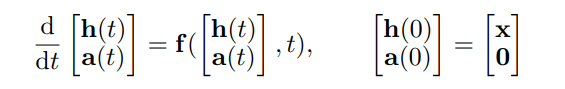
\includegraphics[width=\columnwidth]
   {./Augmented_ODe.png}
   \caption{Activation Function Augmented with Higher Dimensionality \cite{19Dupont}}
   \label{fig:my_label}
\end{figure}


\subsection{Article: How to Train Your Neural ODE}

Beside the adjoint sensitivity method, developed by the authors of the paper \textit{Neural Ordinary Differential Equations},
parallel efforts were also taken to address concerns of high resource usage of back-propagation of NeuralODEs. The paper
\textit{How To Train Your Neural ODE} proposes a method to reduce the computational complexity of back-propagation
in time-series data predictions, by introducing regularization terms to the loss-function \cite{20Finlay}. This allows
for simpler solutions that can be sufficient while limiting NFEs (Number of Function Evaluation) to a reasonable number.
The first regularization term penalty enourages particles to travel with one-dimensional translation by using optimal transport
mapping, while the second regularization term enforces limitations of the vector-field Jacobian to provide force experienced
to be as constant as possible. Such constraint of dynamics allow for simpler solutions with less computational complexities \cite{20Finlay}.

\subsection{A Comparative Derivation of Neural ODE}

Conceptially, NeuralODEs are an extension of Residual Neural Networks. As mentioned previously, the difference between the respective
family of neural networks is the continuos nature of NeuralODEs vs. the discrete nature of Residual Neural Networks. To show the difference,
we will go from one forward-pass calculation of a Residual Neural Network to a NeuralODE.

\textbf{Residual Neural Network}

\[
   h_{t+1} = ReLu(W_{t}h_{t} + b_{t}) + h_{t}
\]

The additional hidden layer term added after the activation function is the residual component of the Residual Neural Network.

Containing the activation function with standard notations, we can rewrite the equation as:

\[
   h_{t} = f(h_{t}, \theta_{t}) + h_{t}
\]

We can convert the following equation to its differential form by expressing it in terms of its limits

\[
   h_{t+1} - h_{t} = f(h_{t}, \theta_{t})
\]

If we reduce the change between one hidden layer to the next to be infinitesimally small, we can express the equation as:

\[
   \frac{h_{t+\delta} - h_{t}}{\delta} = f(h_{t}, \theta_{t})
\]

Taking the limit of $\delta$ and setting it to zero provides us with the differential form of the equation:

\[
   \lim_{\delta \to 0} \hspace*{1ex} \frac{h_{t+\delta} - h_{t}}{\delta} = f(h_{t}, \theta_{t})
\]

\[
   \mathbf{\frac{dh_{t}}{dt} = f(h_{t}, \theta_{t})}
\]

\begin{itemize}
   \item Legend:
   \begin{itemize}
      \item $h_{t}$: Hidden Layer $t$
      \item $W_{t}$: Weight Matrix $t$
      \item $b_{t}$: Bias Vector $t$
      \item $\theta_{t}$: Layer Parameters $t$
      \item $\delta$: Change in Hidden Layer (Infinitesimally Small)
   \end{itemize}
\end{itemize}

\section{Experiment}

\subsection{Defining the Experiment}

An implementation of the Proof-of-Concept NeuralODE is developed. The workflow is modified from a
typical NeuralODE implementation to accomodate visual classification of the MNIST dataset. The same image
classification workflow is performed with a pre-built modified ResNet-18 to classify the MNIST dataset.
Classification accuracy is then compared between the two models from the same testing dataset.

\subsection{Defining Models and Assumptions}

\textbf{Neural ODE}

The NeuralODE implementation is a modified adaptation of the implementation provided by Mikhail Surtsukov. 
Variations were made to the convolutional layer, along with changing the the backpropagation method to use
the adjoint sensitivity method from \textbf{PyTorch} using the Runge-Kutta fixed step solver \cite{19Surtsukov, 23AI}.
The model architecture is as follows:

\begin{itemize}
   \item \textbf{Convolutional Layer (2D)}
   \begin{itemize}
      \item Input: 1 Channel, 28x28 Image
      \item Convolve: 64 Filters, 3x3 Kernel, Stride 1
      \item Norm: Normalize Based on Transport Object [Mean, St. Dev]
      \item ReLU: Activation Function
      \item Convolve: 64 Filters, 3x3 Kernel, Stride 1
   \end{itemize}
   \item \textbf{ODE Layer}
   \begin{itemize}
      \item Input: 64 Filters, 64*12*12 Tensor
      \item Time Update
      \item ODE: ODEFunc
      \begin{itemize}
         \item Convolutional Layer (2D)
         \item ReLU: Activation Function
         \item Statistical Norm [Mean, St. Dev]
         \item Convolutional Layer (2D)
         \item ReLU: Activation Function
         \item Statistical Norm [Mean, St. Dev]
      \end{itemize}
   \end{itemize}
   \item \textbf{Average Pool Layer}
   \item \textbf{Resize: Flatten to 64 Parameters}
   \item \textbf{Fully Connected Layer: 10 Labels}
\end{itemize}

\textbf{ResNet-18}

The ResNet-18 model is a pretrained and pre-built model that is used from the \textbf{PyTorch} Library.
The model architecture generally uses 18 residual layers. ResNet-18 is an adaptation of the
ImageNet architecture used to classify images with 3 channels and 224x224 pixels \cite{23AI}. The model
architecture had to be slightly modified to accomodate the MNIST dataset, which has 1 channel and 28x28 pixels.
The first convolutional layer was edited to have 1 channel \cite{19Shorten}.

\pagebreak

\subsection{Training Method}

\textbf{Hyperparameter Selection}

Hyperparameters [Learning Rate, Epochs, Batch Size] were selected based on standards used for prototyping
convolutional models. The batch size was set to 64, the learning rate was set to 0.0001/.001 for NeuralODE and ResNet-18
respectively, and the number of epochs was set to 10 \cite{19Stoyanov}. 

Initially, the learning rate for NeuralODE was set to 0.001, but the model was not able to converge to a solution
as it was overshooting the argmin of the loss function. The learning rate was reduced to 0.0001, and the model was
able to converge.

As mentioned previously, the \textbf{PyTorch} library was used to train the NeuralODE and ResNet-18 models.
The training method is as follows:
\begin{itemize}
   \item Define Data-Transform Object for ResNet Dimension and Normalization [Mean, St. Dev]
   \item Download MNIST Dataset using PyTorch and save it to directory (Train, Test)
   \item Define Data-Loader Objects for Train and Test Datasets with batch size, and whether to shuffle
   \item Model is defined (For ResNet, modification made to first convolutional layer)
   \item Optimizer [\textbf{Adam}] and Loss Function [\textbf{Cross-Entropy}] is defined
\end{itemize}

\subsection{Results}

Both models were trained for 10 epochs. Both models performed well with accuracies in the high 90th percentile. However,
the ResNet performed better across all epochs, the errors were much more consistent, and the accuracies were higher and consistent.
This could be due to the fact that ResNets are inherently better at image classification than NeuralODEs, In addition, the NeuralODE
did not undergo any hyper-parameter tuning, which could have improved the accuracy of the model. The simpler convolutional layers, along
with the lack of pooling layers could have also contributed to the lower accuracy of the NeuralODE model.



\begin{figure}[H]
   \centering
   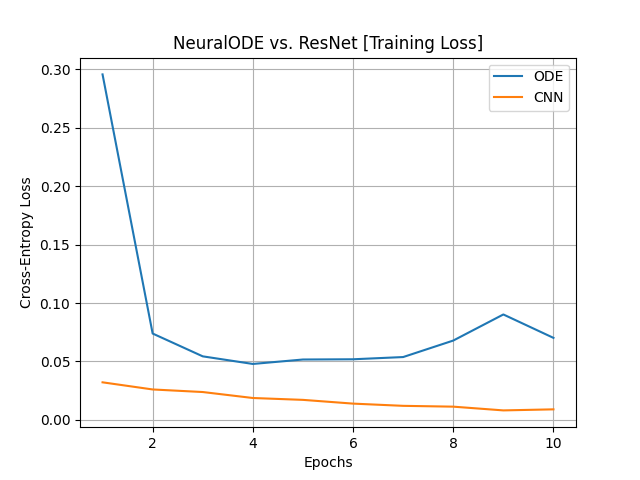
\includegraphics[width=\columnwidth]
   {./TrainingLoss.png}
   \caption{NeuralODE vs. ResNet-18 Training Loss}
   \label{fig:my_label}
\end{figure}

\begin{figure}[H]
   \centering
   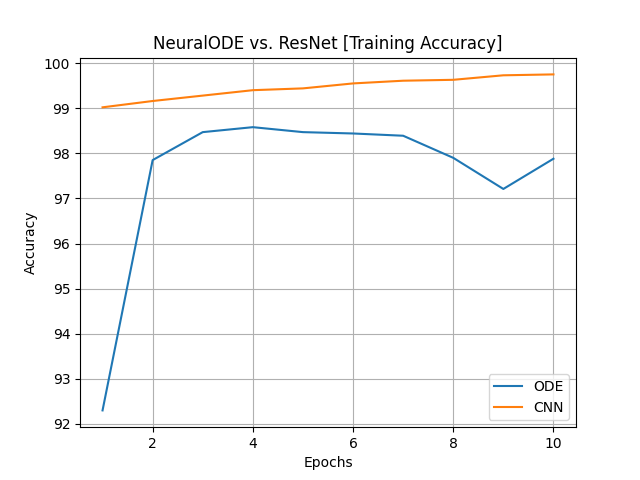
\includegraphics[width=\columnwidth]
   {./TrainingAccuracy.png}
   \caption{NeuralODE vs. ResNet-18 Training Accuracy}
   \label{fig:my_label}
\end{figure}

\begin{figure}[H]
   \centering
   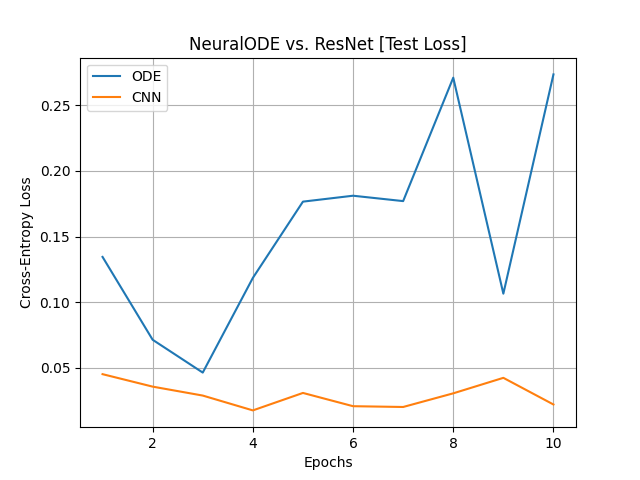
\includegraphics[width=\columnwidth]
   {./TestLoss.png}
   \caption{NeuralODE vs. ResNet-18 Testing Loss}
   \label{fig:my_label}
\end{figure}

\begin{figure}[H]
   \centering
   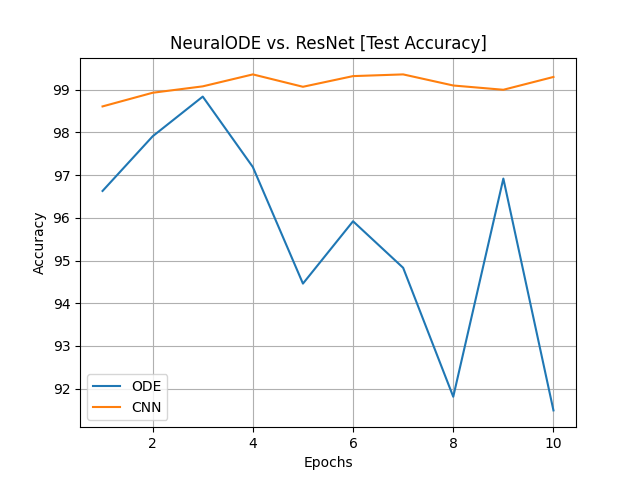
\includegraphics[width=\columnwidth]
   {./TestAccuracy.png}
   \caption{NeuralODE vs. ResNet-18 Testing Accuracy}
   \label{fig:my_label}
\end{figure}

\section{Conclusion}

For the source code that was developed and used in this project, please refer to the following link:

\textbf{Source Code:} https://github.com/Fallensegal/NeuralODE

A short literature review along with a simple implementation of NeuralODEs was presented using available modern tools. 
The NeuralODE model was compared to a ResNet-18 model over the MNIST dataset. Even though both models performed well, 
the ResNet-18 model performed better across all epochs, in addition to it being more consistent.

To build on top of this work. One simple approach would be to understand the effect of hyperparameter tuning on the NeuralODE model.
It could be the fact that NeuralODEs behave differently than ResNets, which could require different standard hyperparameters for optimal
learning. Time series experiments could also be performed to highlight its strenght vs. a convolutional model.

For further expanding on related works, an application of regularization of function dynamics along with the use of the adjoint sensitivity method
for backpropagation could be explored. Such efforts could be fruitful in introducing new variations that are comparitvely resource conservative.




\bibliography{main}
\bibliographystyle{icml2021}

\end{document}


% This document was modified from the file originally made available by
% Pat Langley and Andrea Danyluk for ICML-2K. This version was created
% by Iain Murray in 2018, and modified by Alexandre Bouchard in
% 2019 and 2021. Previous contributors include Dan Roy, Lise Getoor and Tobias
% Scheffer, which was slightly modified from the 2010 version by
% Thorsten Joachims & Johannes Fuernkranz, slightly modified from the
% 2009 version by Kiri Wagstaff and Sam Roweis's 2008 version, which is
% slightly modified from Prasad Tadepalli's 2007 version which is a
% lightly changed version of the previous year's version by Andrew
% Moore, which was in turn edited from those of Kristian Kersting and
% Codrina Lauth. Alex Smola contributed to the algorithmic style files.
